\chapter{Numerical Results}

\section{Filon Method}

The practical implementation of this method is done by using two functions. In accordance with \eqref{oscillatoryIntegral}, $I_1$ and $I_2$ are defined:


\begin{equation}
      I_1=\int_a^{b}dx cos(x)e^{i\omega x}
\end{equation}

\begin{equation}
      I_2 =\int_a^{b}dx (3x+x^2+x^3)e^{i\omega x} 
\end{equation}

These two integrals both have analytical solutions:

\begin{equation}
  I_1=\frac{e^{i a \omega } (\sin (a)+i \omega  \cos (a))-i e^{i b \omega } (\omega  \cos (b)-i \sin (b))}{\omega ^2-1}
\end{equation}

\begin{equation}
  \begin{aligned}
    I_2=\frac{1}{\omega^5}i (&e^{i a \omega } (a (a^3+a+3) \omega ^4+i (4 a^3+2 a+3) \omega ^3-2 (6 a^2+1) \omega ^2-24 i a \omega +24)\\
                             &-e^{i b \omega } (b (b^3+b+3) \omega ^4+i (4 b^3+2 b+3) \omega ^3-2 (6 b^2+1) \omega ^2-24 i b \omega +24))
  \end{aligned}
\end{equation}

\vspace{3in}

\pagebreak

The following numerical results were produced using "filonQuadrature.cpp" code, found in Annex 6.1.

\begin{figure}[H]
  \centering
  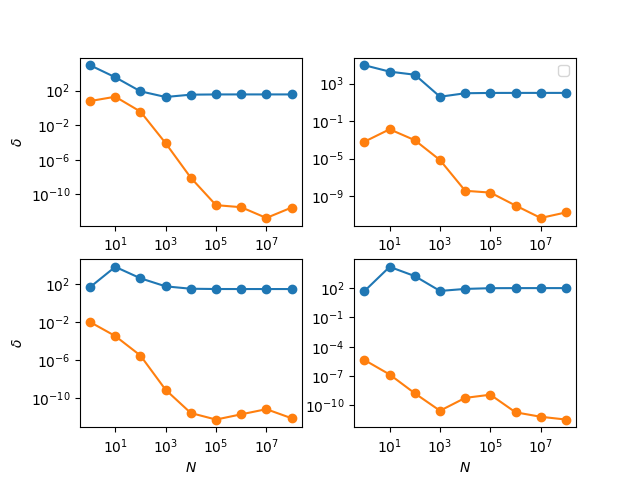
\includegraphics[scale=0.8]{c4/all.png}
  \caption{Relative error of trapezoidal method "$\delta_{Q^T}$" and Filon quadrature "$\delta_{Q^F}$" vs no. of steps $N$ with $a=0,b=100$: (a): $I_1$, $\omega=10$, (b): $I_1$, $\omega=10^3$, (c): $I_2$, $\omega=10$, (d): $I_2$, $\omega=10^3$.}
  \label{figGraphAll}
\end{figure}

The above charts are rendered from numerical data in tables \ref{table1}, \ref{table2}, \ref{table3}, \ref{table4}.  
\vspace{2.5in}


\begin{table}[h!]
    \begin{center}
      \caption{Relative error of trapezoidal method "$\delta_{Q^T}$" and Filon quadrature "$\delta_{Q^F}$" vs no. of steps $N$ on $I_1$ with $a=0,b=100,\omega=10$.}
      \label{table1}
      \pgfplotstabletypeset[
        multicolumn names, % allows to have multicolumn names
        col sep=comma, % the seperator in our .csv file
        display columns/0/.style={
          column name=$N$, % name of first column
          column type={S},string type},  % use siunitx for formatting
        display columns/1/.style={
          column name=$\delta_{Q^T}$,
          column type={S},string type},
        display columns/2/.style={
          column name=$\delta_{Q^F}$,
          column type={S},string type},
        every head row/.style={
          before row={\toprule}, % have a rule at top
          after row={
               & \% & \% \\ % the units seperated by &
              \midrule} % rule under units
              },
          every last row/.style={after row=\bottomrule}, % rule at bottom
      ]{c4/relErrorCosOmega10.csv} % filename/path to file
    \end{center}
  \end{table}


  \begin{table}[h!]
    \begin{center}
      \caption{Relative error of trapezoidal method "$\delta_{Q^T}$" and Filon quadrature "$\delta_{Q^F}$" vs no. of steps $N$ on $I_1$ with $a=0,b=100,\omega=10^3$.}
      \label{table2}
      \pgfplotstabletypeset[
        multicolumn names, % allows to have multicolumn names
        col sep=comma, % the seperator in our .csv file
        display columns/0/.style={
          column name=$N$, % name of first column
          column type={S},string type},  % use siunitx for formatting
        display columns/1/.style={
          column name=$\delta_{Q^T}$,
          column type={S},string type},
        display columns/2/.style={
          column name=$\delta_{Q^F}$,
          column type={S},string type},
        every head row/.style={
          before row={\toprule}, % have a rule at top
          after row={
               & \% & \% \\ % the units seperated by &
              \midrule} % rule under units
              },
          every last row/.style={after row=\bottomrule}, % rule at bottom
      ]{c4/relErrorCosOmega1000.csv} % filename/path to file
    \end{center}
  \end{table}

  \begin{table}[H]
    \begin{center}
      \caption{Relative error of trapezoidal method "$\delta_{Q^T}$" and Filon quadrature "$\delta_{Q^F}$" vs no. of steps $N$ on $I_2$ with $a=0,b=100,\omega=10$.}
      \label{table3}
      \pgfplotstabletypeset[
        multicolumn names, % allows to have multicolumn names
        col sep=comma, % the seperator in our .csv file
        display columns/0/.style={
          column name=$N$, % name of first column
          column type={S},string type},  % use siunitx for formatting
        display columns/1/.style={
          column name=$\delta_{Q^T}$,
          column type={S},string type},
        display columns/2/.style={
          column name=$\delta_{Q^F}$,
          column type={S},string type},
        every head row/.style={
          before row={\toprule}, % have a rule at top
          after row={
               & \% & \% \\ % the units seperated by &
              \midrule} % rule under units
              },
          every last row/.style={after row=\bottomrule}, % rule at bottom
      ]{c4/relErrorPolyOmega10.csv} % filename/path to file
    \end{center}
  \end{table}


  \begin{table}[h!]
    \begin{center}
      \caption{Relative error of trapezoidal method "$\delta_{Q^T}$" and Filon quadrature "$\delta_{Q^F}$" vs no. of steps $N$ on $I_2$ with $a=0,b=100,\omega=10^3$.}
      \label{table4}
      \pgfplotstabletypeset[
        multicolumn names, % allows to have multicolumn names
        col sep=comma, % the seperator in our .csv file
        display columns/0/.style={
          column name=$N$, % name of first column
          column type={S},string type},  % use siunitx for formatting
        display columns/1/.style={
          column name=$\delta_{Q^T}$,
          column type={S},string type},
        display columns/2/.style={
          column name=$\delta_{Q^F}$,
          column type={S},string type},
        every head row/.style={
          before row={\toprule}, % have a rule at top
          after row={
               & \% & \% \\ % the units seperated by &
              \midrule} % rule under units
              },
          every last row/.style={after row=\bottomrule}, % rule at bottom
      ]{c4/relErrorPolyOmega1000.csv} % filename/path to file
    \end{center}
  \end{table}
  \pagebreak

\section{Generalized Filon Method}

The function used in this example is

\begin{equation}
  I_g=\int_a^b dx(x^2+2x^4)e^{i(\omega x+\alpha \sin{\omega_1x})}
\end{equation}

As per the change of variable provided by \eqref{changeOfVariable} and \eqref{changedPhi}, $I'_g$ can be derived as follows


\begin{equation}
  I'_g=\int_{y_{a}}^{y_{b}} dy \frac{x_y^2+2x_y^4}{\omega+\alpha\omega_1cos(\omega_1x(y))}e^{iy}
\end{equation}

There is no analytical solution for $I_g$, therefore the relative error in this example was calculated against
the result obtained from the numerical integration of $I_g$ using
trapezoidal method, at the maximum number of steps $N(10^8)$.\\

The following numerical results were computed using "generalizedFilonQuadrature.cpp" code, found in Annex 6.2, with the parameters 
$\omega=1.0, \omega_1=2.0, \alpha=0.1, a=0, b=10$.

\begin{figure}[H]
  \centering
  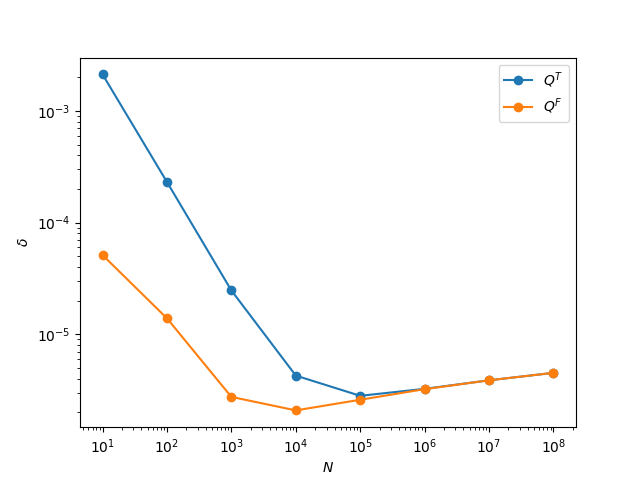
\includegraphics[scale=0.8]{c4/results.png}
  \caption{Relative error of trapezoidal method "$\delta_{Q^T}$" and Filon quadrature "$\delta_{Q^F}$" vs no. of steps $N$,on $I'_g$ against trapezoidal method on $I_g$.}
  \label{figGraphGen}
\end{figure}

The above chart was rendered using the data from \ref{table5}.

\begin{table}[h!]
  \begin{center}
    \caption{Relative error of trapezoidal method "$\delta_{Q^T}$" and Filon quadrature "$\delta_{Q^F}$" vs no. of steps $N$,on $I'_g$ against trapezoidal method on $I_g$.}
    \label{table5}
    \pgfplotstabletypeset[
      multicolumn names, % allows to have multicolumn names
      col sep=comma, % the seperator in our .csv file
      display columns/0/.style={
        column name=$N$, % name of first column
        column type={S},string type},  % use siunitx for formatting
      display columns/1/.style={
        column name=$\delta_{Q^T}$,
        column type={S},string type},
      display columns/2/.style={
        column name=$\delta_{Q^F}$,
        column type={S},string type},
      every head row/.style={
        before row={\toprule}, % have a rule at top
        after row={
             & \% & \% \\ % the units seperated by &
            \midrule} % rule under units
            },
        every last row/.style={after row=\bottomrule}, % rule at bottom
    ]{c4/result.csv} % filename/path to file
  \end{center}
\end{table}


%%% Local Variables:
%%% mode: latex
%%% TeX-master: "../th"
%%% End:
